\chapter{Introduction}
\label{chap:intro}

According to modern quantum theory, to fully describe a (nonrelativistic) system of $N_A$ nuclei and $N_e$ electrons, we must solve the time-dependent Schr\"odinger equation,
\begin{equation}
    \label{eq:schrodinger}
    i \hbar \frac{\partial}{\partial t} \Psi(\bm{x}, t)
    = \hat{H} \Psi(\bm{x}, t)
\end{equation}
where $\bm x=(\bm{r}, \sigma)$, $\bm r\in\mathcal{R}^{3(N_e+N_A)}$ gives the spatial coordinates, and $\sigma$ the corresponding spins. For nuclei with atomic numbers $Z_I$ (positive charge $Ze$), the Hamiltonian operator $\hat H$ may be written

\begin{align}
\begin{split}
\label{eq:theory_of_everything}
\hat H =& -\sum_{I=1}^{N_A}\frac{\hbar^2}{2m_I} \nabla^2_I
+ \frac 1{4\pi\epsilon_0} \frac 12\sum_{I,J=1;I\neq J}^{N_A} \frac{Z_IZ_Je^2}{|\bm R_I-\bm R_J|} \\
&- \sum_{i=1}^{N_e} \frac{\hbar^2}{2m_e} \nabla^2_i
+ \frac 1{4\pi\epsilon_0} \frac 12\sum_{i,j=1;i\neq j}^{N_e} \frac{e^2}{|\bm r_i-\bm r_j|}
- \frac 1{4\pi\epsilon_0}\sum_{i=1}^{N_e} \sum_{I=1}^{N_A} \frac{Z_I e^2}{|\bm r_i-\bm R_I|}
\end{split}
\end{align}
where $N_A$ and $N_e$ are the number of nuclei and electrons, respectively, and we have represented the nuclear coordinates by $\bm R_I$ and the electron coordinates by $\bm r_i$.

Since quantum chemistry and condensed matter sciences are in general concerned with nonrelativistic processes involving electrons and nuclei, this might boldly be called the \emph{theory of everything}.\cite{laughlinTheory2000} Hence, we may be tempted to conclude this dissertation early, but in practice the evaluation of the Hamiltonian in equation \ref{eq:theory_of_everything} is impossible. First, there is no closed form solution of equation \ref{eq:schrodinger} with this Hamiltonian. Second, numerical evaluation of $\hat H$ is far from trivial.

Let's consider a simple example, the Argon atom. Say we want to solve this partial differential equation on a grid. Let's choose a very coarse $10\times 10\times 10$ grid. Then \emph{at each time step} we need to store $10^{3\times (18+18)}=10^{108}$ values, corresponding to all the particle positions and the grid. Considering there are ``only'' $\sim 10^{80}$ atoms in the known universe,\cite{rydenIntroduction2017} this is completely unreasonable.

This system has only 18 electrons and 18 nuclei, a far cry from the $10^{23}$ or higher number of electrons in a typical condensed matter system, for example. Moreover, we have not taken into account floating point precision, or that we would need to calculate this for possibly many time steps. Clearly, drastic approximations and more sophisticated methods are required.

\section{Overview of the Thesis}

This dissertation fits into the field of nonrelativistic electronic structure theory, the branch of quantum chemistry concerned with the description of electrons and their correlation inside molecules and materials. More specifically, this dissertation focuses on high-accuracy (but often high-cost) \emph{ab initio} methodologies, especially \gls{FCIQMC} and \gls{TC}. As such, we will only be discussing small systems consisting of only a few atoms, as they are tractible with a full, all-electron treatment with these methods. In principle, these methods should be able to be embedded \cite{jonesEmbedding2020,christlmaierFull2022} into more large-scale calculations using multiscale techniques, but this is outside the scope of my work. Nevertheless, the work herein is focused on methodologies, and not on particular physical systems.

The outline of the dissertation is as thus:
\begin{itemize}
    \item Chapter \ref{chap:intro} (this chapter) provides a basic overview of electronic structure theory methods and some of its principal concepts. Sections \ref{sec:hf} and \ref{sec:post-hf} in particular are largely based on the appropriate chapters of reference \citenum{helgakerMolecular2014}.
    \item Chapter \ref{chap:explicit} reviews the current works in so-called ``explicitly correlated'' methods, notably the well-established R12/F12 and the recently-reinvigorated \gls{TC}.
    \item Chapter \ref{chap:qmc} provides a basic introduction to \gls{QMC} and how it relates to \gls{FCIQMC}.
    \item Chapter \ref{chap:opt} discusses optimization strategies of Jastrow factors in the context of \gls{TC}.
    \item Chapter \ref{chap:binding} discusses an extension of the methods in the previous chapters to ensure size consistency and success when targeting strongly multireference problems.
    \item Chapter \ref{chap:universal} discusses methods for modular and simple Jastrow factor forms, for easier scalability.
    \item The final chapter, chapter \ref{chap:sumandout}, provides a review and an outlook for the field.
    \item \autoref{chap:pytchint} provides an overview of the software \pytchint developed in the group for evaluation of \gls{TC} integrals.
\end{itemize}


\section{Principal Approximations}

As discussed, to make any progress in electronic structure theory, we must make use of approximations. Of course, we must always be cautious and suspicious when using these, and make sure they are valid for the systems in question. Thankfully, over the course of the last century, a cornucopia of different approximations has been developed to tackle the Schr\"odinger question, some of which will be discussed in this section.

\subsection{The Born-Oppenheimer Approximation}

The most important approximation used in electronic structure theory is the \gls{BOA}.\cite{bornZur1927} The \gls{BOA} relies on the fact that the nuclei are much heavier than the electrons, with the mass of a single proton being almost 2000 times the mass of an electron. As an intuitive picture, we may think of the nuclei as moving much slower than the electrons, which can adapt themselves to the instantaneous positions of the nuclei. In mathematical terms, this means we can take the total wave function to be a product of its nuclear and electronic components,
\begin{equation}
    \Psi_\mathrm{total} = \Psi_\mathrm{nuc} \Psi_\mathrm{elec}.
\end{equation}

Notice that the first two terms of equation \ref{eq:theory_of_everything} are independent of the electronic coordinates and, ipso facto, have no effect on $\Psi_\mathrm{elec}$. This leads to the \emph{electronic Hamiltonian} under the \gls{BOA}, which can be written as
\begin{equation}
\label{eq:elec_hamiltonian}
\hat H_\mathrm{elec} = -\sum_{i} \frac{1}{2} \nabla_i^2 - \sum_{i,I} \frac{Z_I}{r_{iI}} + \sum_{i\gt j} \frac{1}{r_{ij}},
\end{equation}
where we have simplified notation by using miniscule roman letters for the electrons and capital roman letters for the nuclei, and $r_{ij}=|\mathbf{r}_i-\mathbf{r}_j|$ and $r_{iI}=|\mathbf{r}_i-\mathbf{R}_I|$, as well as by using atomic units. That is, the system of units where $\hbar$, $e$, $m_e$, and $4\pi\epsilon_0$ all correspond to the value of $1$.

In the language of second quantisation, equation \ref{eq:elec_hamiltonian} can be written as
\begin{equation}
\label{eq:elec_hamiltonian_2q}
\hat H_\mathrm{elec} = \sum_\sigma\sum_{pq} h^p_{q}a_{p\sigma}^\dag a_{q\sigma}+\frac 12 \sum_{\sigma\tau}\sum_{pqrs} V^{pq}_{rs}a_{p\sigma}^\dag a_{r\tau}^\dag a_{s\tau}a_{q\sigma},
\end{equation}
where $p,q,r,s$ are general spatial-orbital indices, and $a_{p}$ ($a_{p}^\dag$) is the annihilation (creation) operator for an electron in spatial-orbital $p$. $\sigma,\tau$ are the spin indices. These must obey the anti-commutation relations
\begin{equation}
    \{a_{p\sigma},a_{q\tau}^\dag\}
    \mathdef
    a_{p\sigma}a_{q\tau}^\dag + a_{q\tau}^\dag a_{p\sigma}
    =\delta_{pq}\delta_{\sigma\tau}
\end{equation}
\begin{equation}
    \{a_{p\sigma},a_{q\tau}\} = \{a_{p\sigma}^\dag,a_{q\tau}^\dag\} = 0
\end{equation}
so that the electrons satisfy the Pauli exclusion principle.

In equation \ref{eq:elec_hamiltonian_2q}, $h^p_{q}$ is a one-body integral,
\begin{equation}
\label{eq:hij}
h^p_{q} = \int \mathrm{d}^3r\ \phi_p^*(\mathbf{r})\left(-\frac 12 \nabla^2 - \sum_I \frac{Z_I}{|\mathbf{R}_I-\mathbf r|}\right)\phi_q(\mathbf{r})
\end{equation}
and $V^{pq}_{rs}$ is a two-body integral,
\begin{equation}
    V^{pq}_{rs} = \int \mathrm{d}^3r\int\mathrm{d}^3r'\ \phi_p^*(\mathbf{r})\phi_r^*(\mathbf{r}')\frac{1}{|\mathbf{r}-\mathbf{r}'|}\phi_q(\mathbf{r})\phi_s(\mathbf{r}'),
\end{equation}
with a spatial-orbital basis $\{\phi_i(\mathbf{r})\}$.

For our purposes, we neglect the first term of equation \ref{eq:theory_of_everything}, and treat the second term as approximately constant, so $\hat H_\mathrm{nuc} = \sum_{IJ} Z_IZ_Jr_{IJ}^{-1}$. Thus, we are left with the problem of solving the electronic structure problem, which is the subject of this dissertation. Solving the electronic problem for different nuclear positions gives us the potential energy surface.

Note that while chemists and physicists typically talk about the positions of nuclei in a molecule or solid as if they are fixed in place, as will be done in this dissertation, this is really a colloquialism. If the nuclei had an exact position and zero kinetic energy, the \gls{BOA} would be in direct contradiction of the Heisenberg uncertainty principle. Instead, on the timescale of the electrons, due to the much higher mass of nuclei, in the \gls{BOA} we treat the nuclei as approximately localised in a state in which their motion is much slower than that of the electrons (but, importantly, not zero). This keeps the approximation from being in conflict with the fundamental postulates of quantum theory.

The \gls{BOA} is an immensely practical tool as it substantially simplifies our equations, and in many applications it is an excellent approximation. It will be a fundamental assumption throughout the rest of this dissertation, though it need not always be valid in all of quantum chemistry.

While we have done a lot to drastically reduce the complexity of equation \ref{eq:theory_of_everything}, equation \ref{eq:elec_hamiltonian_2q} is still intractible for large system sizes, scaling combinatorially with the size of the Hilbert space, as a function of the system size $N_e$ (henceforth $N$), and the basis set size $M$. Hence, in addition to using a smaller basis, we still need extra approximations and sophisticated methodologies.


\subsection{Core Orbitals}
\label{sec:core_electrons}

In the ground state of a single atom, electrons first occupy the lowest orbitals. The first occupied shells are typically where the electrons are the most tightly bound.\footnote{This neglects symmetries: energy may be higher due to the angular momentum while staying spatially closer to the nucleus.}

Since they tend to be further from the nucleus in an atom, the valence (non-core) orbitals are typically the most affected by the introduction of additional atoms in the system. It is therefore often the valence orbitals that are most important in chemical systems. For this reason, we sometimes ``freeze'' the core orbitals, meaning they remain doubly occupied by electrons, and only correlate the valence orbitals. It is also common to refer to core electrons and valence electrons, meaning those electrons occupying the core and valence orbital space, respectively (though this is technically imprecise language, as electrons are indistinguishable).

Similarly, we may also delete virtual orbitals, typically those of high energy, to further reduce the size of the problem. The remaining space is known as an active space, and is the basic idea of the \gls{CAS} methods.

\subsection{Model Hamiltonians}

In 1929, the surrealist artist Ren\'e Magritte displayed a now-famous painting of a pipe with the caption \emph{Ceci n'est pas une pipe} (French for ``This is not a pipe''). It was meant to depict the idea that the painting itself is in a way treacherous: it may appear to be a pipe, but you cannot stuff it or smoke from it, as it is a representation of a pipe.

In a similar way, physicists and chemists often use \emph{model Hamiltonians}, which do away with aspects of equation \ref{eq:theory_of_everything} that are not expected to be relevant to the problem at hand, resulting in new Hamiltonians that may be considered a representation of equation \ref{eq:theory_of_everything}, much like Magritte's painting.\footnote{We might further argue that all of science can be described this way, as scientific models are always ``mere'' representations of Nature, and are not Nature itself.} Compared to \emph{ab initio} Hamiltonians like equation \ref{eq:elec_hamiltonian_2q}, model Hamiltonians are generally much simpler, but depend on parameters whose values we may not necessarily know a priori.

The most famous model Hamiltonian is the Hubbard model,\cite{Hubbard1963} most typically used to describe electrons in a periodic lattice, and can be written as
\begin{equation}
\label{eq:hubbard}
\hat H_\mathrm{Hubb} = - \sum_{\langle p,q\rangle}\sum_\sigma t_{pq} a_{q\sigma}^\dag a_{p\sigma} + \sum_p U_p\hat n_{p\uparrow}\hat n_{q\downarrow},
\end{equation}
where $\langle p,q\rangle$ denotes nearest neighbour sites, $t_{pq}$ (often taken to be constant, $t$) is a parameter called the hopping amplitude, and $U_p$ (often taken to be constant, $U$) is a parameter called the on-site repulsion. Here we have used a spatial-orbital basis labels $\{p,q\}$ and spin labels $\sigma\in\{\uparrow,\downarrow\}$. $\hat n_{p\sigma}\mathdef a_{p\sigma}^\dag a_{p\sigma}$ is the number operator.

Despite its apparent simplicity, the Hubbard model is a rich model, and has been used to describe a variety of phenomena, from metal-insulator transitions to high-temperature superconductivity. Moreover, it is not always so simple to solve, and has been the subject of much research.\cite{Lieb1968a,liebermannFCIQMC2023}

Let's consider an especially simple version of the model, with only two sites, and open boundary conditions:
\begin{equation}
\label{eq:hubbard_h2}
\hat H_\mathrm{Hubb} = - t\sum_{\sigma}(a_{1\sigma}^\dag a_{2\sigma} + a_{2\sigma}^\dag a_{1\sigma}) + U(\hat n_{1\uparrow}\hat n_{1\downarrow}+\hat n_{2\uparrow}\hat n_{2\downarrow}).
\end{equation}
We could use this as an approximate description of the H$_2$ molecule, where the electrons are restricted to only the lowest 1s orbitals. Compared to equation \ref{eq:theory_of_everything}, this is a tremendously easy problem now.

Of course, when solving a problem using a model Hamiltonian, we must be careful in choosing the correct one. In particular, the exact solution to the Hubbard model in one dimension\cite{Lieb1968a} does not appear to be in agreement with the \emph{ab initio} solution of a one-dimensional chain of hydrogen atoms.\cite{Motta2017,Motta2020}

\section{The Variational Principle}
\label{sec:variational_principle}

One way of finding approximations to the lowest energy eigenstate of a quantum problem like that of equation \ref{eq:elec_hamiltonian_2q} is the variational method. Several methods discussed in this dissertation build on the variational method, and the variational method itself is based on the variational principle, which states\cite{sakuraiModern2017} for any ``trial wave function'' $\ket{\tilde\Psi}$ and Hermitian operator (such as the electronic Hamiltonian) $\hat H$,
\begin{equation}
    \label{eq:variational_principle}
    \frac{\bra{\tilde\Psi}\hat H\ket{\tilde\Psi}}{\braket{\tilde\Psi}}
    \ge E_0 \mathdef  \frac{\bra{\Psi}\hat H\ket{\Psi}}{\braket{\Psi}}
\end{equation}
where $E_0$ is the lowest eigenvalue (e.g. the ground state energy). That is, the energy of $\ket{\tilde\Psi}$ is an upper bound of the exact energy of the system.

To prove this, consider an expansion of $\ket{\tilde\Psi}$ terms of the exact eigenkets $\ket k$ of $\hat H$, so that $\hat H\ket k = E_k\ket k$ and $\ket{\tilde\Psi}=\sum_kc_k\ket k$. Then
\begin{align}
\label{eq:var_proof}
    \begin{split}
    \frac{\bra{\tilde\Psi}\hat H\ket{\tilde\Psi}}{\braket{\tilde\Psi}}
    &=
    \frac{\sum_{kk'}c_k^*c_{k'}\bra{k}\hat H\ket{k'}}{\sum_{kk'}\bra{k}\ket{k'}c_k^*c_{k'}}\\
    &= \frac{\sum_k|c_k|^2(E_k-E_0)}{\sum_k|c_k|^2} + E_0 \\
    &\ge E_0
\end{split}
\end{align}
where, in going from the first to the second line, we used the orthonormality of the eigenbasis $\{\ket k\}$ and that the left- and right-eigenvectors are the same. That is, we used the fact the $\hat H$ is a Hermitian operator. This is an important observation for future discussions, such as in section \ref{sec:tc}.

\section{The Schr\"odinger Equation as a Matrix Problem}
\label{sec:matrix}

Implicit in the operator algebra of the fermionic creation and annihilation operators $a^\dag$ and $a$ in equation \ref{eq:elec_hamiltonian_2q} is the Pauli exclusion principle: we cannot have two or more fermions occupying identical states. In the context of electronic structure theory and this dissertation, the fermions and states in question are electrons and orbitals, respectively. This handles the antisymmetry requirement of the fermionic wave function, $\hat P_{ij}^\sigma\Psi = -\Psi$, where $\hat P_{ij}^\sigma$ permutes the $i$th and $j$th electrons with spin $\sigma$.

Our wave function can hence be expanded by a linear combination of \glspl{SD},
\begin{equation}
    \label{eq:SD_expansion}
\Psi = \sum_i c_i \ket{D_i},
\quad \text{where } \ket{D_i} =
\frac 1{\sqrt{N!}}\left|
    \begin{matrix}
        \chi_1(\bm x_1) & \chi_1(\bm x_2) & \cdots & \chi_1(\bm x_N)\\
        \chi_2(\bm x_1) & \chi_2(\bm x_2) & \cdots & \chi_2(\bm x_N)\\
        \vdots & \vdots & \ddots & \vdots\\
        \chi_N(\bm x_1) & \chi_N(\bm x_2) & \cdots & \chi_N(\bm x_N)\\
    \end{matrix}
 \right|
\end{equation}
for a spin-orbital basis $\{\chi_p(\bm x_q)\}$. A spin-orbital is typically written as a product of a spatial part and a spin part, e.g. $\chi(\bm x) = \phi(\bm r)\omega(\sigma)$.

Given such a finite spin-orbital basis of size $2M$ ($M$ spatial orbitals with 2 different spins each),\footnote{We assume here the same number of spin-$\uparrow$ and spin-$\downarrow$ orbitals for simplicity, though it need not always be the case.} the \gls{SD} expansion is also finite. Therefore, we may write $\hat H$ as a square matrix and equation \ref{eq:elec_hamiltonian_2q} as an eigenvalue equation,
\begin{equation}
\label{eq:eval_eqn}
\hat H\Psi = E\Psi.
\end{equation}

Note, however, that in order to make this a finite-dimensional matrix eigenvalue problem, we needed to use a finite spin-orbital basis. Thus, $E$ in equation \ref{eq:eval_eqn} is not the true ground state energy of the system, but indeed only an approximation within that basis set. This is the case even if we were to solve equation \ref{eq:eval_eqn} exactly. In order to get the true ground state energy, we need to reach the \gls{CBS}, i.e. $M\to\infty$.

With equation \ref{eq:eval_eqn}, we have transformed the hopelessly intractible partial differential equation \ref{eq:theory_of_everything} into a finite algebraic eigenvalue problem, which is much better suited for solving on a computer.

If we have $N_\uparrow$ spin-up electrons and $N_\downarrow$ spin-down electrons, we then have
\begin{equation}
\label{eq:scaling}
|\mathcal{H}| = {M \choose N_\uparrow}{M\choose N_\downarrow}
\end{equation}
where $|\mathcal{H}|$ denotes the size of the Hilbert space, and we have assumed that the number of spin-up orbitals $M$ is equal to the number of spin-down orbitals. Here, ${n\choose r}=\frac{n!}{r!(n-r)!}$ is a binomial coefficient.

The combinatorial scaling is still unfavourable. For a closed-shell system with 20 electrons in 20 orbitals, $|\mathcal{H}|=3.41\times 10^{10}$. Assuming we wish to have double precision,\footnote{A double precision floating-point number has 1 bit for the sign, 11 bits for the exponent, and 52 bits for digits in the number (known as the mantissa or significand).\cite{ascherFirst2011} This resolves to 64 bits or 8 bytes.} to store the whole matrix we would need about $10^{23}$ bytes, or 100 zettabytes. So, while we've substantially reduced the complexity of the problem, it is still extremely demanding. More approximations are therefore needed.

\subsection{Orbitals}
\label{sec:orbitals}

Orbitals (and spin-orbitals), a term already used in this text, describe the spatial distribution (and in the case of spin-orbitals, also the spin) of a single electron. We assume that spatial orbitals form an orthonormal set, and that they form a complete space for an arbitrary wave function. However, in theory to have a \gls{CBS} would mean needing an infinite number of basis functions. In practice, we must of course have a finite basis, and so this naturally leads to a hierarchy of basis sets, where the typically larger basis sets are both more expensive and more accurate.

Many different basis set families exist, but among the most popular are those due to Dunning and coworkers.\cite{dunningGaussian1989} Additionally, many different basis set extrapolation techniques have also been developed.\cite{fellerEffectiveness2011,halkierBasisset1998,halkierBasisset1999,helgakerBasisset1997,jensenBasis1999,pansiniExtrapolation2016,petersonBenchmark1994,woonBenchmark1994}

Strictly speaking, any kind of set of functions can be used as a basis set, as long as they are a complete set. However, in practice we may broadly categorise them into two groups: \glspl{STO} and \glspl{GTO}.

The exact solution for the Hydrogen atom is the Slater-type function $\frac 1{\sqrt{\pi}} \e^{-r}$, and similarly we know that molecular orbitals also decay as $\sim e^{-\zeta r}$.

However, these \glspl{STO} are difficult to work with, as integrals of the form
\begin{equation}
    \label{eq:two-body-integral}
\int\d^3r_1\int d^3r_2\ \phi_p^*(\bm r_1)\phi_r^*(\bm r_2)\frac 1 {r_{12}}\phi_q(\bm r_1)\phi_s(\bm r_2)
\end{equation}
are routinely needed.

Therefore, \glspl{GTO} have been developed,\cite{boysElectronic1950} which have the form $\e^{-\alpha r^2}$. \glspl{GTO} are much easier to handle, as the product of a gaussian is also a gaussian, and the integral of a gaussian is exactly known, so equations like \ref{eq:two-body-integral} have known solutions. With this comes a tradeoff, since we know \glspl{STO} more faithfully capture the form of molecular orbitals, but \glspl{GTO} are much better suited for computations. For this, the most common basis sets typically use a linear combination (or ``contraction'') of gaussians fitted to a \gls{STO}. An illustration is shown in figure \ref{fig:sto-gto}.

It must be noted, however, that \glspl{STO} and \glspl{GTO} have different asymptotic behaviour for $r\to\infty$ and $r\to 0$. The latter in particular will be discussed in section \ref{sec:cusp}.

\begin{figure}[htbp]
    \centering
    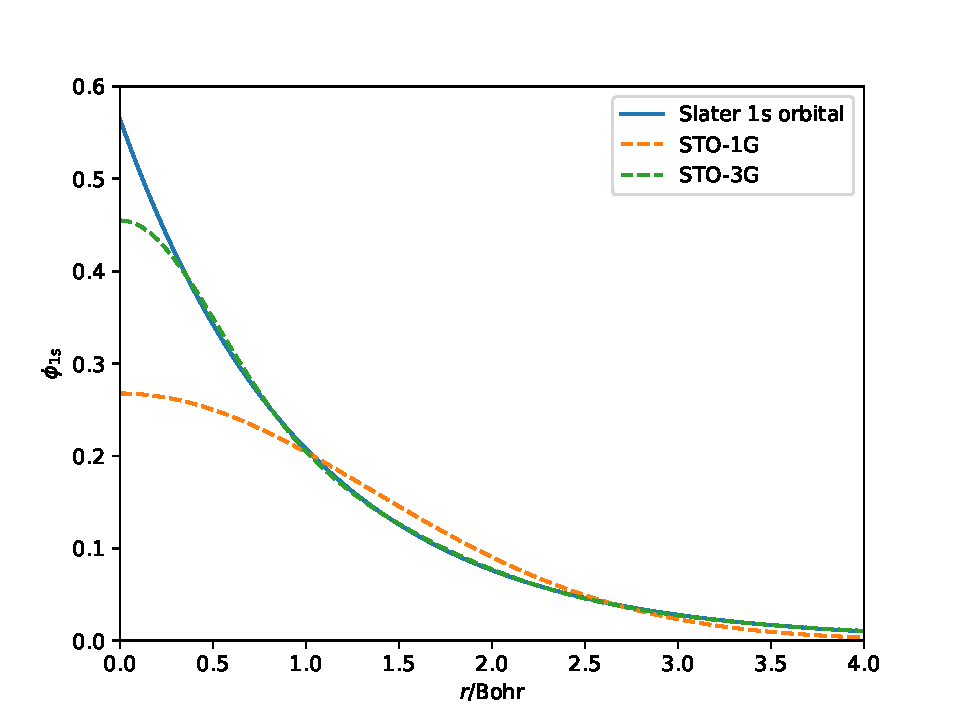
\includegraphics{figures/intro/gto-sto.pdf}
    \caption{Illustration of an $s$-type orbital and the fitted gaussians (STO-$x$G means $x$ gaussians are used to approximate the \gls{STO}). Note that for much of the curve, there is good agreement, but not for the short- and long-range. The short-range behaviour in particular leads to complications, and is the focus of the methods discussed in chapter \ref{chap:explicit}. The long-range behaviour is typically less of a problem, since the integrals we are interested in typically decay with $r$. Fitting parameters for the gaussians were taken from reference \citenum{szaboModern2012}.}
    \label{fig:sto-gto}
\end{figure}

\subsection{Density Matrices}
\label{sec:density-matrices}

The \gls{1RDM} is defined by its matrix elements
\begin{equation}
    \gamma_{pq} = \bra{\Psi}a_q^\dag a_p \ket{\Psi},
\end{equation}
or written in a spin-orbital basis:
\begin{equation}
    \label{eq:one-rdm}
    \gamma(\bm x_1, \bm x_2) = \sum_{pq} \phi_q(\bm x_2)^*\phi_p(\bm x_1) \gamma_{pq}
\end{equation}

Similarly, the \gls{2RDM} is defined as
\begin{equation}
    \label{eq:two-rdm}
    \Gamma_{pqrs} = \bra{\Psi}a_s^\dag a_r^\dag a_q a_p \ket{\Psi}.
\end{equation}

Any one- and two-electron Hermitian operator $\Omega$ can be written (in a spin-orbital basis) as
\begin{equation}
    \label{eq:rdm-expectation}
    \bra{\Psi}\Omega\ket{\Psi} = \sum_{pq} \gamma_{pq}\Omega_{pq} + \sum_{pqrs} \Gamma_{pqrs}\Omega_{rpsq}.
\end{equation}

\subsection{Electron Correlation}
\label{sec:correlation}

% note: primarily using haettig F12 review paper here
Two variables are independent (or uncorrelated) if the joint probability distribution is the product of their expected values, i.e.
\begin{equation}
    P(\bm x_1, \bm x_2) = P(\bm x_1)P(\bm x_2).
\end{equation}

By Bayes' theorem,\cite{hastieElements2009,bayesLII1997} this can be rewritten in terms of the conditional probability,
\begin{equation}
    P(\bm x_1|\bm x_2) = \frac{P(\bm x_1, \bm x_2)}{P(\bm x_2)} = \frac{P(\bm x_1)P(\bm x_2)}{P(\bm x_2)} = P(\bm x_1).
\end{equation}
The variables are said to be correlated if the above is not true.

In the case of electronic structure, the variables in question are $\bm x \mathdef (\bm r, \sigma)$, the spatial coordinates and spin of the electrons. Therefore, when we speak of electron correlation, we are referring to these relations. Furthermore, as electrons are indistinguishable, for every pair $(\bm x_1, \bm x_2)$,
\begin{align}
    &P(\bm x_1) = P(\bm x_2) = \frac 1N \rho(\bm x) \\
    &P(\bm x_1, \bm x_2) = \frac 1{N(N-1)} \rho(\bm x_1, \bm x_2)
\end{align}
where $\rho(\bm x)$ is the electron density and $\rho(\bm x_1, \bm x_2)$ is the probability of finding electrons at $(\bm x_1, \bm x_2)$ simultaneously, known as the pair density,
\begin{align}
    \rho(\bm x) &= N\int \d^3x_2 \cdots \d^3x_N \Psi^*(\bm x, \bm x_2, \bm x_3, \cdots, \bm x_N)\Psi(\bm x, \bm x_2, \bm x_3, \cdots, \bm x_N) \\
    \rho(\bm x_1, \bm x_2) &= N(N-1)\int \d^3x_2 \cdots \d^3x_N \Psi^*(\bm x_1, \bm x_2, \bm x_3, \cdots, \bm x_N)\Psi(\bm x_1, \bm x_2, \bm x_3, \cdots, \bm x_N).
\end{align}

There are two key sources of electron correlation: Fermi correlation, which arises from the fact that electrons obey Fermi statistics, i.e. the wave function is antisymmetric with respect to exchange of $\bm x_1$ and $\bm x_2$, and Coulomb correlation, which arises from the fact that electrons repel each other.

\section{The Hartree-Fock Method}
\label{sec:hf}

The typical starting point to most \emph{ab initio} electronic structure methods is the \gls{HF} method.\cite{hartreeWave1928,fockNaherungsmethode1930,slaterNote1930} The key approximation in \gls{HF} is that we treat the exact $N$-body wave function solution as approximately a single \gls{SD}.\footnote{More precisely, the \gls{HF} approximation is to treat the wave function as a single configuration. In the context of this dissertation, that configuration will always be a \gls{SD}.} Then, we variationally (see section \ref{sec:variational_principle}) optimise the energy of the system with respect to parameters pertaining to the spin-orbitals. We will refer to this \gls{SD} as $\ket{\Phi_0}$.

Then, for some arbitrary initial configuration $\ket 0$,
\begin{equation}
\ket{\Phi_0} = \e^{-\kappa} \ket 0.
\end{equation}
Here,
\begin{equation}
\kappa = \sum_{PQ} \kappa_{PQ}a_P^\dag a_Q
\end{equation}
is an anti-Hermitian operator (i.e. $\kappa_{PQ}^* = -\kappa_{QP}$) whose matrix elements $\kappa_{PQ}$ are the orbital rotation coefficients and will be the variational parameters. The anti-Hermiticity of $\kappa$ ensures that the orbital rotation $\e^{-\kappa}$ is unitary. Here we use the convention that capital $P,Q$ denote spin-orbital indices.

With $\braket{\Phi_0}=1$, we want
\begin{equation}
E_\mathrm{HF} = \min_{\kappa_{PQ}}\bra{\Phi_0}\hat H\ket{\Phi_0}.
\end{equation}
This is a nonlinear equation, and hence the parameters $\kappa_{PQ}$ must be determined iteratively. Since $\e^{-\kappa}$ is unitary, the orthonormality of the spin-orbitals is preserved, $\bra{\phi_P}\ket{\phi_Q} = \delta_{PQ}$.

The \gls{HF} method can also be understood as a mean-field theory. That is, we treat the $N$-body problem as $N$ one-body problems, where a single electron is in an effective ``averaged'' potential from the other $N-1$ electrons. This effective one-body Hamiltonian is known as the Fock operator,
\begin{equation}
    \label{eq:fock-operator}
    f = \sum_{PQ} f^P_{Q} a_P^\dag a_Q.
\end{equation}

The Fock operator $f$ may be written as
\begin{equation}
    f = h + V_\mathrm{eff}
\end{equation}
where the Fock potential's matrix elements (in spatial-orbital basis) are $V_{\mathrm{eff},pq}=\sum_{i\in\mathrm{occ}}(V^{pq}_{ii}-V^{pi}_{iq})$.

The Hartree-Fock orbitals, which ultimately dictate the parameters for the minimisation procedure, are determined by diagonalising the Fock matrix,
\begin{equation}
    f^p_{q} = \epsilon_p\delta^p_{q}
\end{equation}
where the eigenvalues $\epsilon_p$ are known as the orbital energies.

Since $f$ itself depends on the orbitals, the solution must be determined self-consistently. Hence \gls{HF} is often referred to as a \gls{SCF} method.

Often, the orbitals for the $\uparrow$ and $\downarrow$ electrons are restricted to be the same. This is known as the \gls{RHF} method. Otherwise, we might instead use the \gls{UHF} method, where they are treated independently. However, since this breaks spin symmetry, we might have spin contamination. \Gls{ROHF} is a variant that can treat open-shell systems which \gls{RHF} otherwise would not be able to treat while remaining an eigenstate of the $S^2$ (total spin) operator.

\subsection{Correlation Energy}

The correlation energy (for a given basis set) is defined as the difference between the exact energy and the \gls{HF} energy,
\begin{equation}
E_\mathrm{corr} = E_\mathrm{exact} - E_\mathrm{HF}.
\end{equation}
It should be noted, however, that despite this name the \gls{HF} method captures Pauli exchange, and hence does actually correlate electrons. Nevertheless, we typically neglect this when we speak of ``correlation energy''.

Similarly, the Coulomb hole is defined as the remaining part of the wave function that is not captured by the \gls{HF} method,
\begin{equation}
    \Psi_\mathrm{hole} = \Psi_\mathrm{exact} - \Psi_\mathrm{HF}.
\end{equation}

\subsection{The Roothaan-Hall Equations}

The Roothaan-Hall equations are a matrix representation of the \gls{HF} approximation.\cite{roothaanNew1951,hallMolecular1997} Given a basis set, typically \glspl{GTO}, the Roothaan-Hall equations are given by the generalised eigenvalue problem,
\begin{equation}
    FC = SC\bm\epsilon
\end{equation}
where $C$ is a matrix of coefficients, $F$ is the Fock matrix (which depends on $C$), $S$ is the overlap matrix (which reduces to the identity matrix for orthonormalised bases), and $\bm\epsilon$ is a diagonal matrix of orbital energies. The Roothaan-Hall equations are obtained by expanding the unknown \glspl{MO} in a basis of known functions, typically \glspl{AO}.

Since this representation is in matrix form, instead of in terms of derivatives and integrals, it is more amenable to conventional computational techniques.

\section{Post-Hartree-Fock Methods}
\label{sec:post-hf}

While the \gls{HF} method is convenient and can be used efficiently to solve for many electrons, it is oftentimes not sufficient to describe the electronic structure of a molecule. To account for the remaining correlation, numerous post-Hartree-Fock methods (that is, methods run after \gls{HF}) have been formulated, some of which are described in this section.

Correlation energy is typically categorised as either dynamical or static, although their effects are not mutually exclusive and so sometimes the distinction can be hazy.

Dynamical correlation is remaining correlation that arises due to the instantaneous repulsion from the motion (dynamics) of the electrons.

Static correlation, on the other hand, is related to the degeneracy or near-degeneracy of configurations. In general, to accurately describe a system with strong static correlation, a so-called multi-reference method is needed. As will be seen in chapter \ref{chap:binding}, static correlation plays a big role for molecules at dissociation.

We therefore have two ``axes'' on which to approach the exact solution to equation \ref{eq:elec_hamiltonian_2q}:
\begin{itemize}
    \item The basis set chosen, where going to a larger basis set (in a systematic way) improves the result, e.g. cc-pVDZ to cc-pVTZ to cc-pVQZ, until eventually reaching the \gls{CBS} limit.
    \item The ``hierarchy of theories'' where the more accurate the method, the closer to the \gls{FCI} limit (discussed below). Many post-Hartree-Fock methods can be systematically improved, for example by considering additional excitations in a coupled cluster method.
\end{itemize}

\begin{figure}[htbp]
    \centering
    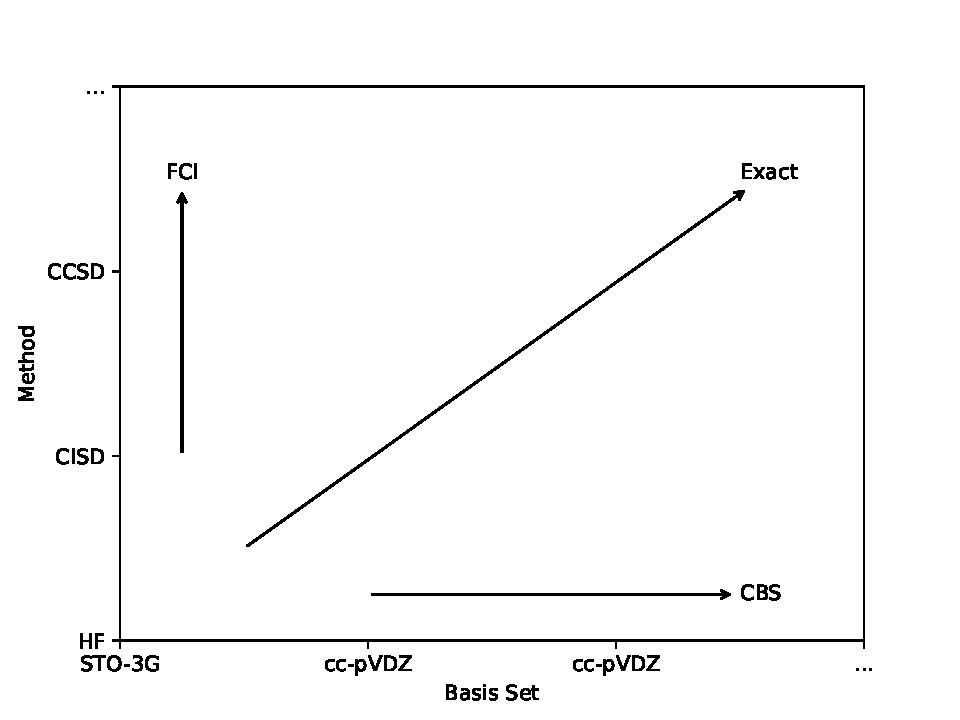
\includegraphics[width=0.8\textwidth]{figures/intro/hierarchies.pdf}
    \caption{A sketch for the hierarchy of theories and basis sets. There are two axes on which to systematically improve until reaching the exact solution to the time-independent Schr\"odinger equation under the \gls{BOA}: increasing basis set size (x axis) and increasing the level of theory (y axis). For most of this dissertation, we assume to be at or close to the highest level of theory (the FCI limit), as we mostly employ \gls{FCIQMC}. We therefore focus on methods of rapidly converging to the \gls{CBS} limit without the inherently expensive process of adding more basis functions.}
    \label{fig:hierarchies}
\end{figure}

% For so-called ``weakly-correlated'' electron systems, the \gls{HF} method or a modest improvement thereof is sufficient. However, for ``strongly-correlated'' electron systems, the \gls{HF} method can fail completely, not even describing the system qualitatively correctly.


\subsection{Configuration Interaction}
\label{sec:ci}

\Gls{CI} is perhaps the most conceptually straightforward post-Hartree-Fock method. Instead of using a single \gls{SD}, we approximate the wave function as a linear combination of \glspl{SD}. That is,
\begin{equation}
\ket{\Phi_\mathrm{CI}} = \sum_p c_p\ket{D_p}
\end{equation}
where $\ket{D_p}$ is a \gls{SD}. This may alternatively be written\footnote{We adopt the common notation convention where $i,j,k,...$ denote occupied orbitals, $a,b,c,...$ virtual (or unoccupied) orbitals, and $p,q,r, ...$ unspecified.}
\begin{equation}
\label{eq:ci}
\ket{\Phi_\mathrm{CI}} = (\one + \sum_\sigma\sum_{ia}c_i^a\hat a_{a\sigma}^\dag\hat a_{i\sigma} +
\sum_{\sigma\tau}\sum_{ijab}c_{ij}^{ab} a_{a\sigma}^\dag a_{b\tau}^\dag a_{i\tau} a_{j\sigma}+...)\ket{\Phi_0}
\end{equation}
where the number of terms in the sum depends on how many excitations we consider, i.e. how far we truncate the \gls{CI} expansion. The energy and wave function are then found as the lowest eigenvalue and corresponding eigenvector, respectively, of the Hamiltonian written in the basis of these \glspl{SD}. This can be done, for example, by exact diagonalisation. If all possible excitations are considered, then we have reached the \gls{CBS} limit, and the solution is exact within that basis set.

\begin{figure}[htbp]
    \centering
    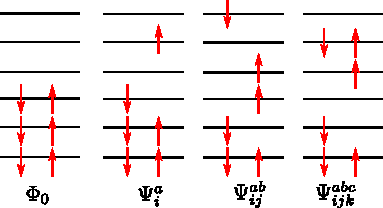
\includegraphics{figures/intro/configurations.pdf}
    \caption{Illustration of a \gls{RHF} reference and examples of single-, double-, and triple-excitations. The method CISDT, for example, would consider all determinants of the forms illustrated.}
    \label{fig:excitations}
\end{figure}

There are some important limitations to this method, however. Perhaps most notable is that the \gls{CI} method is not size consistent. For two noninteracting systems $A$ and $B$, we expect the composite system $A+B$ to have energy equal to the sum of that for $A$ and $B$, i.e. $E_{A+B}=E_A+E_B$. However, within a truncated \gls{CI} method, this is not the case\footnote{Of course, in \gls{FCI} we necessarily have size consistency, since we have the exact solution for the basis set.}, due to the additive ansatz \ref{eq:ci}.

Additionally, if we wish to go to the \gls{FCI} limit and ensure size consistency and accurate results, we once again have bad scaling, as discussed in section \ref{sec:matrix}. However, there exist sparse diagonalisation routines that need not store the entire matrix $H$, such as the Davidson,\cite{davidsonIterative1975} Lanczos,\cite{lanczosIteration1950} and Arnoldi\cite{arnoldiPrinciple1951} (for non-Hermitian $H$) methods, which target the ground state and need to store only a fraction of the matrix. Still, these scale with the size of the eigenvector, which is still prohibitively expensive for large systems. A more practical approach to reaching \gls{FCI} accuracy will be discussed later in section \ref{sec:fciqmc}, where we discuss the \gls{FCIQMC} algorithm.

\subsection{Multi-Configurational Self-Consistent Field}

As a generalisation of the \gls{HF} method, \gls{MCSCF} is particularly well-suited for problems with static correlation.\cite{helgakerMolecular2014,eadeDirect1981,roosNew1972} As in \gls{HF}, we minimise the electronic energy with respect to variational parameters; however, now we also simultaneously minimise with respect to expansion coefficients for a set of configurations (e.g. \glspl{SD}). i.e. consider the MCSCF wave function
\begin{equation}
\ket{\kappa,\bm c} = e^{-\kappa}\sum_ic_i\ket{D_i},
\end{equation}
where $\kappa$ is familiar from HF, and the $c_i$ coefficients farmiliar from \gls{CI}. In MCSCF, we optimise
\begin{equation}
E_\mathrm{MCSCF} = \frac{\bra{\kappa,\bm c}H\ket{\kappa,\bm c}}{\bra{\kappa,\bm c}\ket{\kappa,\bm c}}.
\end{equation}

Like in HF, the variational parameters appear nonlinearly and must be optimised iteratively. Determining an appropriate set $\{\ket{D_i}\}$ tends to be challenging, and even for small systems generating an MCSCF wave function can prove intractible.

\subsubsection{Complete Active Space Self-Consistent Field}
One ``flavour'' of \gls{MCSCF} that has proven particularly successful is \gls{CASSCF}.\cite{olsenCASSCF2011,roosComplete1980,siegbahnComparison1980,siegbahnComplete1981} In CASSCF, instead of inspecting individual configurations, we consider a set of configurations that satisfy a set of criteria. In particular, we partition the orbitals into three sets: the core, active, and virtual (unoccupied) regions. The core orbitals, as alluded to in section \ref{sec:core_electrons}, are approximated to be doubly occupied. The virtual orbitals are approximated to always be unoccupied. The active orbitals are the remaining orbitals, which can have occupations between 0 and 2.

The MCSCF expansion is found by considering all possible excitations of the active electrons in the active space. Notice that in the limit of an empty active space, we recover the \gls{HF} method, and in the limit of an active space containing all orbitals, we recover the \gls{FCI} method.

% might want to include a graphic for CAS space partitioning (or not idk)

\subsection{Perturbation Theory}
\label{sec:perturbation-theory}

Perturbation theory is a set of approximate mathematical methods for solving problems involving small disturbances (perturbations) to a problem with a known solution (the unperturbed problem). If these perturbations are not too large, then the solution of the perturbed problem is close to that of the unperturbed problem, and can be expressed as the solution of the unperturbed problem plus some corrections. Perturbation theory fails, however, if the perturbation is large.

\subsubsection{Rayleigh-Schr\"odinger}

Perturbation theory applied to time-independent problems is sometimes referred to as Rayleigh-Schr\"odinger perturbation theory.\cite{sakuraiModern2017,rayleighTheory1945,schrodingerQuantisierung1926} Consider a Hamiltonian,
\begin{equation}
H_\mathrm{PT} = H_0 + \lambda H',
\end{equation}
where $H_0$, referred to as the unperturbed Hamiltonian, $\lambda$ is an arbitrary (real) parameter controlling the strength of the perturbation, and $H'$ is the perturbation. We assume that we know the exact solution to $H_0$, such that we have all eigenstates $\{\ket{\Psi_n^{(0)}}\}$ and their corresponding eigenvalues $\{E_n^{(0)} \}$.

To obtain the solution to the true Hamiltonian $H$, we expand in terms of the perturbation $\lambda$,
\begin{equation}
\ket{\Psi_n} = \sum_{k=0}^\infty \lambda^k\ket{\Psi_n^{(k)}}
\end{equation}
and
\begin{equation}
E_n = \sum_{k=0}^\infty \lambda^kE_n^{(k)}.
\end{equation}
Since in this work we are generally interested in the ground state, we are typically targeting $n=0$.

By inserting these expansions into the time-independent Schr\"odinger equation, we equate terms of the same order in $\lambda$, which leads to the corrections to the energy and wave function. We may then truncate the expansion to some order. This allows for a systematically improvable result.

\subsubsection{M{\o}ller-Plesset}

M{\o}ller-Plesset perturbation theory\cite{mollerNote1934} is a special case of Rayleigh-Schr\"odinger perturbation theory, and is the variant most commonly seen in quantum chemistry.

In M{\o}ller-Plesset perturbation theory, the unperturbed Hamiltonian is chosen to be the Fock operator \ref{eq:fock-operator}. The perturbed Hamiltonian is known as the fluctuation potential and is the difference between the true Coulomb interaction and the effective one-electron potential discussed in section \ref{sec:hf}.

That is,
\begin{equation}
    H_0 = f, \hspace{10pt} H' = \sum_{i<j} r_{ij}^{-1}-V_\mathrm{eff} = H-H_0.
\end{equation}
If we apply Rayleigh-Schr\"odinger perturbation theory, we find the zeroth order wave function to be the \gls{HF} wave function,
\begin{equation}
    \ket{\Psi_0^{(0)}} = \ket{\Phi_0}, \hspace{10pt}
    f\ket{\Phi_0} = \underbrace{\sum_i\epsilon_i}_{E_0^{(0)}}\ket{\Phi_0}
    % , \hspace{10pt} E^{(0)} = E_\mathrm{HF}.
\end{equation}
where we have also identified the zeroth-order energy as the sum of orbital energies $E^{(0)}=\sum_i\epsilon_i$. With a bit more busywork, we get
\begin{align}
    E^{(1)} &= \bra{\Psi_0^{(0)}}H'\ket{\Psi_0^{(0)}} = \bra{\Phi_0}H'\ket{\Phi_0} \\
    E^{(2)} &=
    \sum_{n>0} \frac{|\bra{\Psi_n^{(0)}}H'\ket{\Psi_0^{(0)}}|^2}{E_0^{(0)}-E_n^{(0)}} =
    -\sum_{i>j,a>b}\frac{|\bra{\Phi_{ij}^{ab}}H'\ket{\Phi_0}|^2}{\epsilon_a+\epsilon_b-\epsilon_i-\epsilon_j},
\end{align}
where $\ket{\Phi_{ij}^{ab}}=a_a^\dag a_b^\dag a_ia_j\ket{\Phi_0}$ is a doubly-excited state with respect to the HF wave function, and $\epsilon_a+\epsilon_b-\epsilon_i-\epsilon_j = E_0^{(0)} - E_n^{(0)}$ is the energy difference between two eigenstates of the Fock operator.

Some features worth noting about M{\o}ller-Plesset perturbation theory:
\begin{itemize}
    \item The sum of zeroth- and first-order energies is the HF energy: $E_\mathrm{HF} = E_0^{(0)} + E_0^{(1)}$.
    \item By the variational principle, $E_0^{(0)}<E_n^{(0)}$ for all $n>0$ (except for degenerate ground states), so $E_0^{(2)}<0$, i.e. the energy always decreases.
    \item If the ground state is degenerate, the term diverges. It might be possible to lift the degeneracy by a change of basis, however.
    \item If the \gls{HF} solution is already a good approximation for the system, then M{\o}ller-Plesset perturbation theory can provide surprisingly good (and size consistent) results. Hence, this method is typically only applicable to single-reference problems (i.e. those without strong static correlation).
\end{itemize}

While higher-order approaches exist and see use, the most popular is \gls{MP2}, due to its excellent compromise between cost and accuracy. That is, for only a little extra work after a successful \gls{HF}, applying \gls{MP2} can improve our results considerably.

\subsection{Coupled Cluster Theory}

The lack of size consistency in \gls{CI} theory arises from the linear ansatz in section \ref{sec:ci}. By instead using an exponential ansatz, we arrive at one of the most successful theories in electronic theory, \gls{CC}.\cite{cizekCorrelation1966,cizekCorrelation1971,paldusTimeIndependent1975,shavittManyBody2009} While the methods presented here are inherently single-reference and build on a single \gls{SD}, multi-reference generalisations to \gls{CC} theory exist and are the study of active research.\cite{aotoInternally2016,evangelistaPerspective2018,hanauerPilot2011,jankowskiApplicability1992,jeziorskiCoupledcluster1981,kohnImproved2020} Therefore, the presented ``flavours'' of \gls{CC} are generally expected to fail for systems with strong static correlation.

\subsubsection{Standard Coupled Cluster}

To ensure a multiplicatively-separable wave function, we use a multiplicative ansatz,
\begin{equation}
    \label{eq:cc-ansatz}
\ket{\Psi_\mathrm{CC}} = \e^T\ket{\Phi_0},
\end{equation}
where $\ket{\Phi_0}$ is the reference (typically \gls{HF}) wave function, and $T$ is the cluster operator. The cluster operator is defined $T = T_1 + T_2 + T_3 + \cdots$, where $T_n$ is the $n$-body cluster operator, made up of all possible $n$-body excitations, for example, $T_1 = \sum_\sigma\sum_{i,a}t_{ia}a_{a\sigma}^\dag a_{i\sigma}$ for the one-body cluster operator, and $T_2 = \sum_{\sigma\tau}\sum_{i<j,a<b}t_{ij}^{ab}a_{a\sigma}^\dag a_{b\tau}^\dag a_{j\tau} a_{i\sigma}$ for the two-body cluster operator.

It is worth noting that \gls{CC} and \gls{CI} are identical, differing only in their parametrisation, when neither are truncated. They both provide \gls{FCI}-level accuracy.

By inserting equation \ref{eq:cc-ansatz} into the time-independent Schr\"odinger equation and pre-multiplying by $\e^{-T}$, we obtain

\begin{align}
    \bra{\Phi_0}\e^{-T} H \e^T\ket{\Phi_0} &= E \\
    \label{eq:cc-schrodinger}
    \bra{\Phi_{ij...}^{ab...}}\e^{-T} H \e^T\ket{\Phi_0} &= 0
\end{align}
where $\ket{\Phi_{ij...}^{ab...}}$ is a $n$-body excitation with respect to the reference wave function.

Note, however, that these equations do not rely on the Variational Principle. Instead of minimising a functional, we solve equations \ref{eq:cc-schrodinger} for the amplitudes, which give the energy. While we still cannot reasonably always include all excitations in the cluster operator $T$, due to the multiplicative ansatz, even if we truncate the cluster operator, we get size-consistent results. In particular, any truncated CC wave function ansatz will contain contributions from all determinants in Fock space. The simplest CC truncation commonly used is the \gls{CCSD} method. In a sense, \gls{CCSD} and any other truncated CC method is an approximation for \gls{FCI} where the coefficients are not approximated to be zero (like in \gls{CI}) but instead the higher-order excitations terms are generated from the lower-order excitation terms in a size-consistent fashion.

CC theory owes much of its success to its high accuracy at a reasonable cost. \gls{CCSD} and \gls{CCSDT} in particular scale as $\mathcal{O}(M^6)$ and $\mathcal{O}(M^8)$ respectively, with $M$ the number of spatial orbitals. Every additional set of excitations incurs an additional factor of $\mathcal{O}(M^2)$ scaling.

\subsubsection{Distinguishable Cluster Theory}

The more recently-developed \gls{DCSD} method's central philosophy is removing irrelevant or nonphysical terms while maintaining many of CC's desireable properties, such as size consistency.\cite{katsCommunication2013}

This method was shown to give quantitatively better results than standard CC for a variety of systems, and qualitatively correct results for systems where CC can fail spectacularly, such as the N$_2$ binding curve. Since its first publication, \gls{DC} has been extended to explicitly-correlated F12 theory,\cite{katsAccurate2015} \gls{EOM},\cite{rishiExcited2017} tailored coupled cluster,\cite{vitaleFCIQMCTailored2020} and more.

\subsubsection{Combining Coupled Cluster with Perturbation Theory}

It is possible to avoid the computationally-expensive scaling of CC somewhat, by treating some terms perturbatively. The most famous of these is the \gls{CCSD(T)} method,\cite{raghavachariFifthorder1989} in which the single- and double-excitations are treated fully, whereas the triple-excitations are treated as perturbations, as in section \ref{sec:perturbation-theory}.

\gls{CCSD(T)} scales as $\mathcal{O}(M^7)$ and for the price provides extremely accurate results. The perturbative correction is a step that is applied only once at the end of a \gls{CCSD} calculation. This is why sometimes this method is referred to as the ``gold standard'' of quantum chemistry.

% \subsection{Density Matrix Renormalisation Group}
